\chapter{Propiedades catalíticas de nw de ZnO wurtzita.}

Hoy en día, las caldas solares sensibilizadas por colorante (DSSC) son los sistemas más investigados para la conversión de energía solar en electricidad, particularmente para su implementación en dispositivos donde se requieren bajos costos y buen rendimiento. Las DSSC de mayor rendimiento utilizan electrolitos líquidos a base de disolventes orgánicos, los cuales tienen el inconveniente de una alta presión de vapor y un severo impacto medioambiental. Además, varios disolventes orgánicos son tóxicos y/o explosivos, lo que limita seriamente sus aplicaciones prácticas en DSSC debido a problemas de seguridad. A pesar de que se han propuesto varias alternativas a los disolventes orgánicos \cite{Li2014,Pringle2013}, el problema que a veces se ignora es la contaminación de la celda por medio de humedad/agua que afecta tanto al rendimiento de la celda como a la estabilidad a largo plazo. De hecho, siempre están presentes trazas de agua en la solución electrolítica y en los poros/huecos de la película del electrodo SC, que eventualmente se introducen durante el ensamblaje de la celda o al operar en condiciones ambientales. En consecuencia, es fundamental averiguar cual es el papel específico del agua como componente en las DSSC, si se trata de un envenenamiento o la palabra clave para el éxito, lo cual se logra a partir del análisis minucioso de todos los fenómenos establecidos en el medio acuoso. Entonces, consideramos muy interesante y sorprendente el hecho de que, en los últimos años, la comunidad científica ha orientado sus investigaciones en dirección a las DSSC fabricados con electrolitos a base de agua, haciendo estudios tanto experimentales \cite{Husmann2018,Cassone2018} como teóricos con TD-DFT \cite{Angelis2011}. De esta manera se podrían lograr fácilmente costos reducidos, no inflamabilidad, volatilidad reducida y compatibilidad ambiental mejorada. Las modificaciones de fotoanodos, la introducción de nuevos aditivos y tensioactivos, la selección de pares redox específicamente concebidos, la preparación de cátodos adecuados y la estabilización de electrolitos han conducido progresivamente a la fabricación de DSSC 100$\%$ acuosas ({\bf DSSC acuosas}, ver figura \ref{dssc_acuosa}). Lograr un alto rendimiento en una celda completamente acuosa representa un avance significativo para las DSSC y devuelve la atención a su propósito inicial: la realización de un sistema fotosintético artificial capaz de convertir la energía de la luz solar visible en electricidad, mediante el uso de un disolvente único, agua, el solvente de la vida. Por último y no menos importante el uso del agua como componente clave puede representar un gran paso hacia su amplia difusión en el mercado. 



\begin{figure}[!htb]
\centering
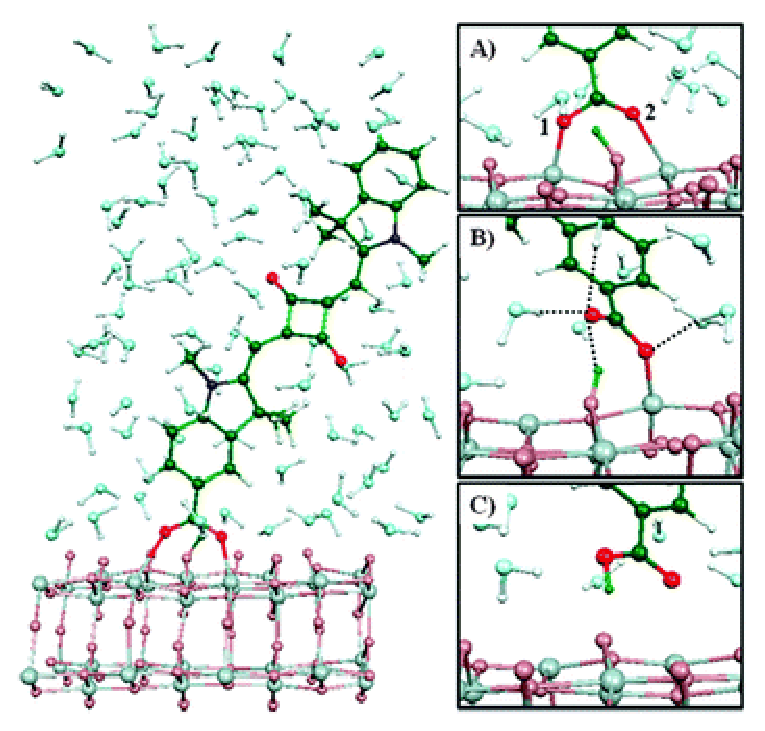
\includegraphics[height=6cm]{cap6/figs/dssc_acuosa.eps}
\caption{Imagen de una DSSC aquosa: Squaraina adsorbida sobre un slab de anatasa, rodeada por 90 moléculas de agua. En las imágenes del lado derecho, se muestran las configuraciones relevantes muestreadas durante el estudio TD-DFT: A) configuración inicial bidentada con átomos de oxígeno etiquetados, B) configuración monodentada y C) colorante disociado. Las líneas punteadas en B) representan enlaces de hidrógeno al grupo carboxílico. Extraído de \cite{Angelis2011}} 
\label{dssc_acuosa}
\end{figure}



De acuerdo al trabajo publicado por Bella \textit{et al} \cite{Bella2015}, parece que la calidad de la interfase fotoanodo/electrolito afecta negativamente la eficiencia de las DSSC acuosas en comparación con las basadas en disolventes orgánicos. La hidrofilicidad excesiva de la superficie sensibilizada con el colorante favorece la desorción de la molécula sensibilizadora disminuyendo así la fotocorriente y la estabilidad en el tiempo; por otro lado, los colorantes altamente hidrófobos no permiten la humectabilidad completa del electrodo lo que, a su vez, da como resultado un proceso de regeneración menos efectivo para los electrolitos acuosos. Las estrategias más efectivas hacia DSSC acuosas realistas incluyen el uso de complejos de cobalto como mediadores redox, colorantes hidrófobos combinados/funcionalizados con tensioactivos o débilmente hidrófilos obtenidos mediante la modificación de sensibilizadores ya disponibles y contraelectrodos tolerantes al agua con una amplia superficie. Sin embargo, el estudio de las DSSC acuosas se encuentra en una etapa temprana y aún faltan estudios comparativos que puedan mejorar en gran medida el conocimiento de estos sistemas.

El objetivo de este capítulo es estudiar al agua como componente electrolítico en sistemas agua - nw de ZnO wurtzita y las interacciones que ocurren entre ambas especies utilizando distintos niveles de teoría: dinámica molecular (LAMMPS), DFT (Quantum expresso) y DFTB (dftb+). 


\section{Complejos 1H$_2$O + nw ZnO wurtzita}

En primer lugar se realizaron simulaciones de sistemas nw-H$_2$O utilizando solamente 1 molécula de agua. Las superceldas que se utilizaron en los cálculos son las que se muestran en la figura \ref{supercelda}, las cuales se construyeron apilando 2 celdad unidad o 2 nw$_1$ en el eje z. Es importante aclarar que las estructuras de celda unidad son las mismas que utilizamos en el capítulo 5. El tamaño de la supercelda debe ser lo suficientemente grande como para que la molécula de agua no interaccione con su imagen periódica y además el costo computacional no sea muy elevado especialmente al utilizar Quantum Espresso (\textbf {QE}).

La molécula de agua se puede unir a la superficie del nw de diversas maneras. En esta tesis propusimos 2 configuraciones: C$_A$ y C$_B$ (ver figura \ref{supercelda}), en C$_A$ el O del agua interacciona con un Zn superficial del nw (O$_w$--Zn$_{nw}$) mientras que en C$_B$ uno de los H del agua interacciona con un O superficial del nw (H$_w$--O$_{nw}$). Ambos Zn y O superficiales tienen número de coordinación 3 lo que los vuelve más reactivos con respecto a los otros átomos que se encuentran dentro del nw con número de coordinación 4. 


\begin{figure}[!htb]
\centering
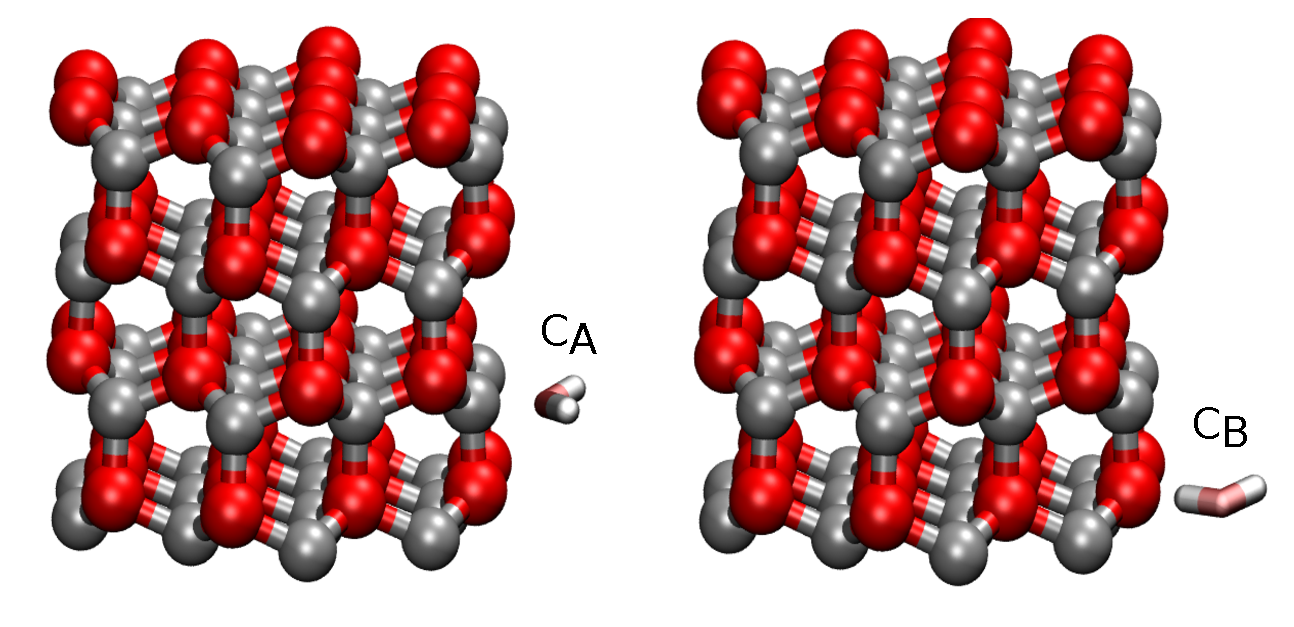
\includegraphics[height=5cm]{cap6/figs/conf_ca_cb.eps}
\caption{Superceldas utilizadas para los cálculos. C$_A$ y C$_B$ son las configuraciones propuestas para la unión del agua a la sueprficie del nw.} 
\label{supercelda}
\end{figure}


\subsection{Análisis configuracional}

Ambos sistemas con distinta configuración del agua fueron relajados utilizando LAMMPS, QE y dftb+. 
Se utilizó el potencial ReaxFF para los cálculos realizados con el software LAMMPS ya que según la literatura se han encontrado buenos resultados en concordancia con los experimentos y el pseudopotencial pbe en QE. 


Una manera típica de buscar mínimos estables es simplemente relajando desde las distintas configuraciones. Sin embargo, antes de realizar este procedimiento decidimos dejar que la dinámica molecular (DM), a través de LAMMPS, pruebe varias configuraciones hasta quedarse con la más estable a medida que disminuye la temperatura. En este método que se llama \textbf{templado simulado}, el sistema explora la superficie de energía potencial y a medida que disminuye la temperatura se va ubicando en mínimos locales. De esta manera, al llegar a aproximadamente 0 K, el sistema se encuentra en un mínimo que puede ser el mínimo global o un mínimo local muy estable. El gráfico de la figura \ref{rampa} muestra la rampa de temperatura (300 K-$0.05$ K) que se utilizó para el templado a medida que avanza la dinámica. 


\begin{figure}[!htb]
\centering
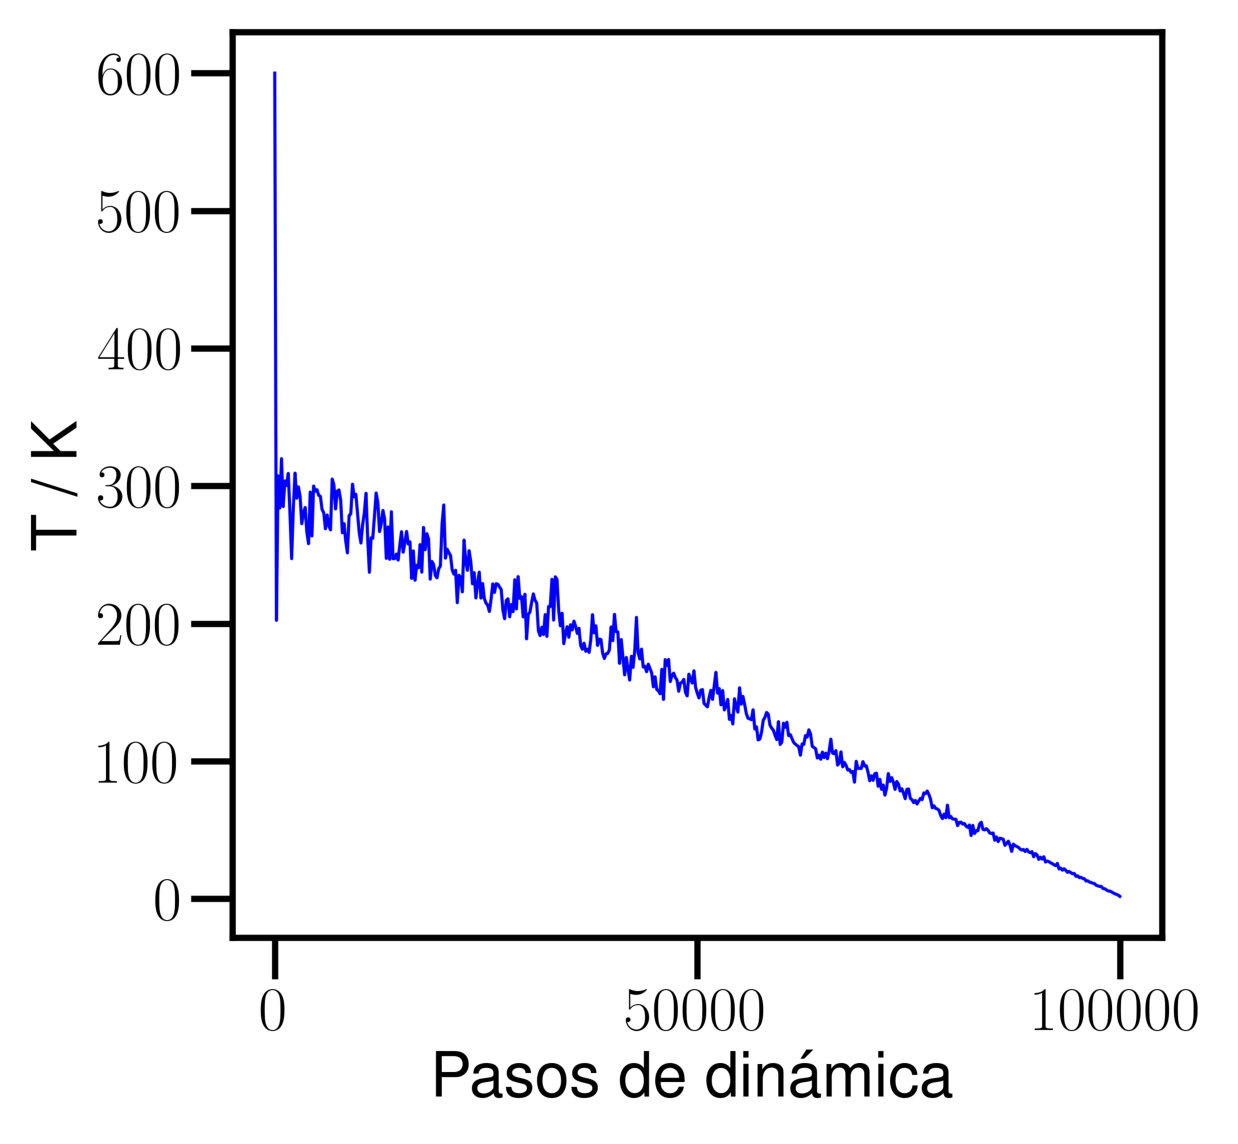
\includegraphics[height=8cm]{cap6/figs/temps_steps.eps}
\caption{Gráfico de temperatura vs pasos de dinámica para la relajación de C$_A$ y C$_B$ en LAMMPS utilizando templado simulado} 
\label{rampa}
\end{figure}

Luego del templado simulado se realiza una relajación en z a 0 K con LAMMPS. Las configuraciones obtenidas con dinámica molecular fueron relajadas nuevamente por dftb+ y QE, respectivamente en z a 0 K. Los resultados obtenidos de las optimizaciones de geometría se muestran en la figura \ref{relax}. 


\begin{figure}[!htb]
\centering
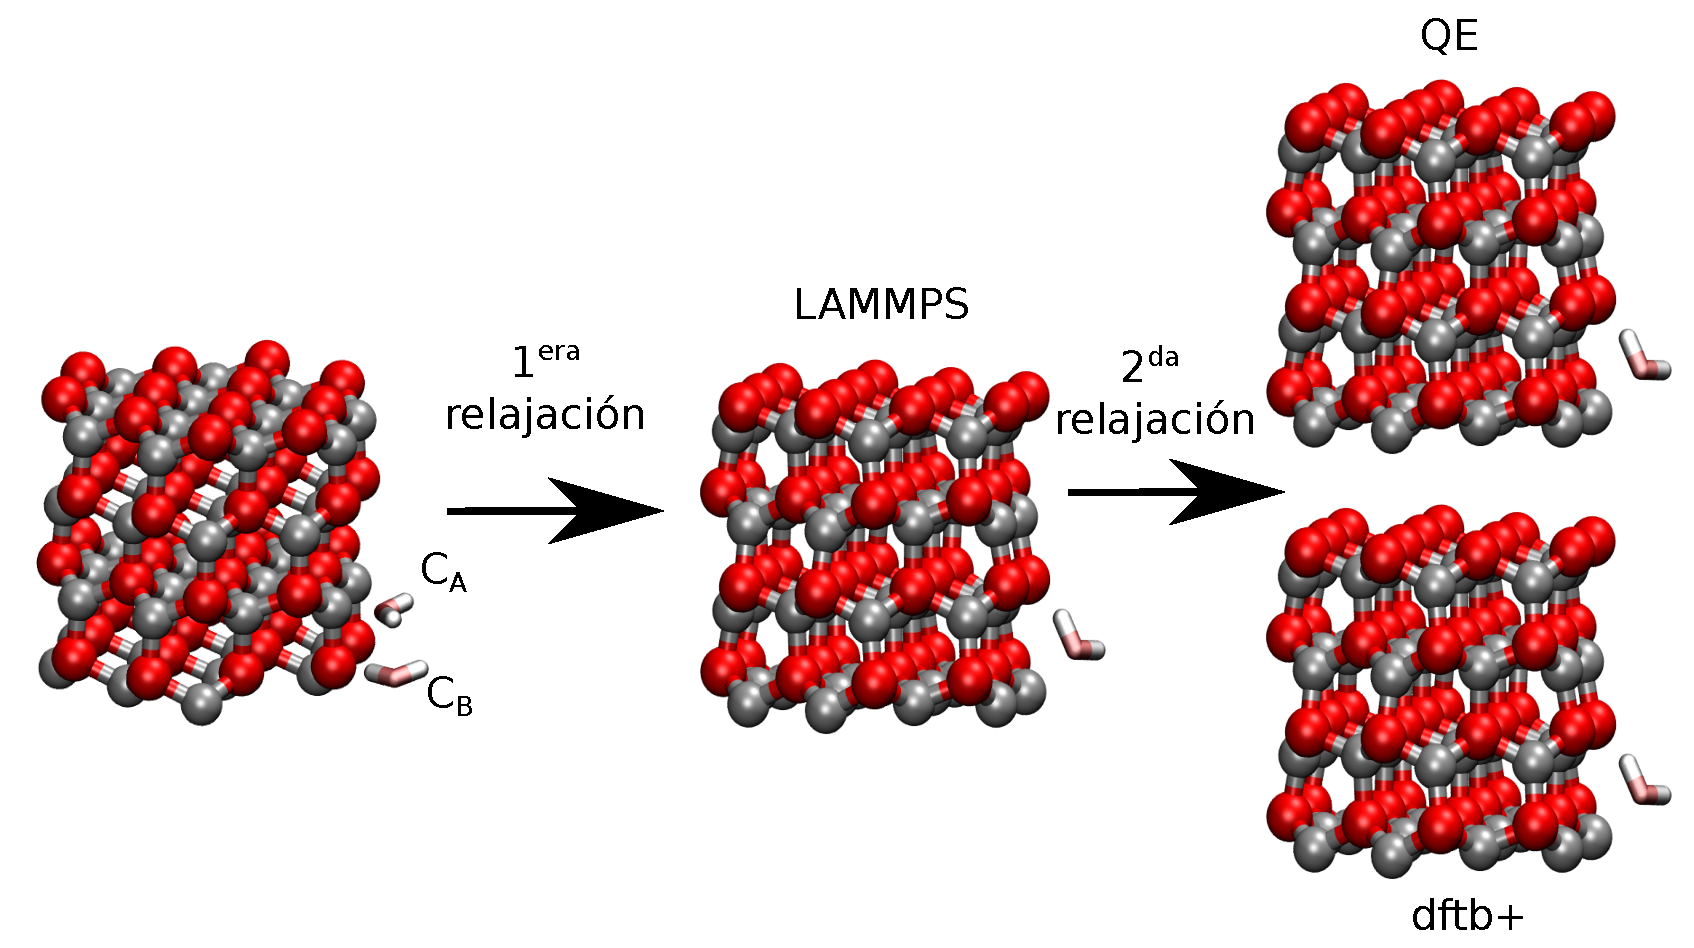
\includegraphics[height=8.5cm]{cap6/figs/relax.eps}
\caption{Relajaciones de las configuraciones C$_A$ y C$_B$ utilizando primero LAMMPS y luego QE y dftb+ } 
\label{relax}
\end{figure}

La relajación con DM para los sistemas C$_A$ y C$_B$, respectivamente, dio como resultado dos configuraciones idénticas y distintas con respecto a C$_A$ y C$_B$. Luego al relajar por segunda vez con QE y con dftb+ se obtuvo una estructura prácticamente igual a la que encontró LAMMPS como lo demuestra a simple vista la figura \ref{relax}. Para corroborar la hipótesis de que los tres métodos encontraron la misma configuración más estable para el sistema 1H$_2$0-nw, se compararon por un lado los diámetros y alturas de las celdas unidad del nw y por otro las distancias H$_w$--O$_{nw}$ y Zn$_{nw}$--O$_w$ que muestran el posicionamiento de las moléculas de agua con respecto al nw. Todas las mediciones se realizaron para cada una de las estructuras obtenidas luego de las relajaciones con los distintos software.

\begin{table}[!htb]
  \caption{Comparación de diámetro y altura de las celdas unidad de los sistemas 1H$_2$0-nw relajados en z utilizando LAMMPS, dftb+ y QE}
  \label{tabla_distancias_nw}
  \centering
  %\resizebox{14cm}{!} {
  \begin{tabular}{ c  c  c  }
   \hline
   \multicolumn{1}{c}{} & \multicolumn{1}{c}{Diámetro ({\AA})} & \multicolumn{1}{c}{Altura ({\AA})} \\
   \hline
    LAMMPS & $9.80$ & $5.47$\\
    dftb+ & $9.98$ & $5.46$\\ 
    QE & $9.88$ & $5.40$\\ 
    \hline
 \end{tabular}
 %}
  \end{table}

La tabla \ref{tabla_distancias_nw} compara solo las estructuras de los nw de los sistemas 1H$_2$0-nw. Los valores obtenidos con QE son tomados como referencia ya que los cálculos con DFT han demostrado tener una buena concordancia con resultados experimentales para sistemas SC??. De acuerdo a esta expresión, las 3 estructuras de nw pueden considerarse equivalentes debido a que el diámetro y la altura de las celdas unidad obtenidas con dftb+ y LAMMPS difieren en menos de $0.2$ {\AA} con respecto a QE, error que se considera razonable. Los valores de diámetro que arroja LAMMPS son más próximos a la referencia en comparación con dftb+ mientras que este último muestra valores de altura de la celda unidad más cercanos a QE. 


\begin{figure}[!htb]
\centering
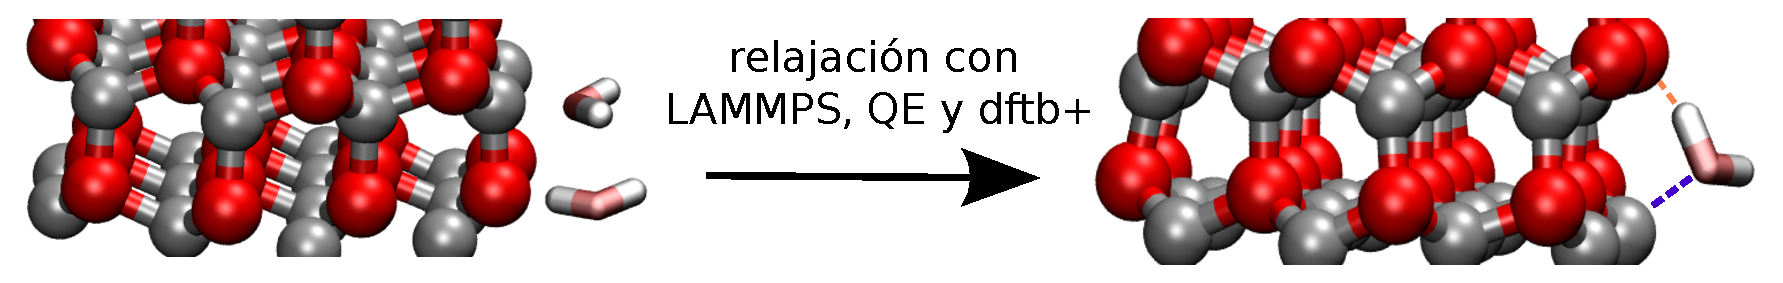
\includegraphics[height=2.1cm]{cap6/figs/antes_despues_relax_cur.eps}
\caption{(\textbf {Izquierda}) configuraciones iniciales (C$_A$-C$_B$) y (\textbf {derecha}) configuración final en todos los casos (C$_C$)} 
\label{CC}
\end{figure} 

\begin{table}[!htb]
 \caption{Comparación de las distancias H$_w$--O$_{nw}$ y Zn$_{nw}$--O$_w$ de los sistemas 1H$_2$0-nw relajados con LAMMPS, dftb+ y QE}
 \label{tabla_distancias_agua}
 \centering
 %\resizebox{14cm}{!} {
 \begin{tabular}{ c  c  c  }
  \hline
  \multicolumn{1}{c}{} & \multicolumn{1}{c}{Distancia \textcolor{orange}{\textbf{H}}$_w$--\textcolor{orange}{\textbf{O}}$_{nw}$ ({\AA})} & \multicolumn{1}{c}{Distancia \textcolor{blue}{\textbf{Zn}}$_{nw}$--\textcolor{blue}{\textbf{O}}$_w$ ({\AA})} \\
  \hline
    LAMMPS & $1.56$ & $2.30$\\
    dftb+ & $1.78$ & $2.13$\\ 
    QE & $1.64$ & $2.12$\\ 
    \hline
 \end{tabular}
 %}
\end{table} 
  
La tabla \ref{tabla_distancias_agua} compara las distancias H$_w$--O$_{nw}$ y Zn$_{nw}$--O$_w$ para los sistemas 1H$_2$0-nw optimizados utilizando tres niveles de teoría. En este caos tampoco se observa una tendencia en los valores obtenidos, sin embargo, las diferencias con respecto a QE también son menores a $0.2$ eV. Podemos decir, entonces, que las tres estructuras obtenidas de las relajaciones de C$_A$ y C$_B$ con distintos software son equivalentes entre si, lo cual significa que los métodos conciden en que la configuración del sistema 1H$_2$0-nw ZnO más estable es la que se muestra en la figura \ref{CC} (C$_C$).
Los resultados nos permiten validar los métodos LAMMPS y dftb+ en cuestión, otorgando credibilidad a los cálculos de relajación en sistemas H$_2$0-nw ZnO. Por otro lado observamos que la configuración mas estable encontrada por los 3 software tiene en cuenta ambas interacciones simultáneamente, es decir:  H$_w$-O$_{nw}$ y Zn$_{nw}$-O$_w$, en lugar de considerar las interacciones por separado como planteamos al inicio del capítulo.

En último lugar, para investigar el tipo de unión que que se establece entre el adsorbato (agua) y la superficie del SC (nw) realizamos cálculos de energía de adsorción, E$_ad$, para la configuración C$_C$ (ver tabla \ref{tabla_ead})

La E$_{ad}$ se obtuvo de acuerdo a la siguiente ecuación:

\begin{equation}
 E_{ad} = E_{T(H_20 + nw)} - E_{T(nw)} - E_{T(H_20)}
\end{equation}

donde E$_{T(H_20 + nw)}$ es la energía total del sistema 1H$_2$0-nw, E$_{T(nw)}$ la energía total del nw de ZnO y E$_{T(H_20)}$ de la molécula de agua. 

  
\begin{table}[!htb]
  \caption{Energías de adsorción para C$_C$ calculadas mediante los 3 métodos analizados}
  \label{tabla_ead}
  \centering
  \begin{tabular}{ c  c }
   \hline
   \multicolumn{1}{c}{} & \multicolumn{1}{c}{E$_{ad}$ (eV)}\\
   \hline
   & C$_C$\\
   \hline
    LAMMPS & $-1.02$ \\
    dftb+ & $-1.15$ \\ 
    QE & $-0.81$ \\
    \hline
   \end{tabular}
\end{table}  
  
Se observan valores negativos de E$_{ad}$ para las 3 simulaciones, reflejando una unión fuerte entre el adsorbato (H$_2$O) y el adsorbente (nw). Tomando a QE como el método más preciso, dftb+ y LAMMPS sobrestiman la interacción H$_2$O-nw. 
  
  
\section{Complejos nH$_2$O + nw ZnO wurtzita}

En esta sección se realizó en primer lugar un cálculo de DM para el sistema: nw de ZnO wurtzita + primer cilindro de solvatación de agua (\textbf {1slv agua-nw}) a 300 K.  El 1$^{er}$ cilindro de solvatación se seleccionó realizando un corte a una distancia de $2.33$ {\AA} desde la superficie del alambre en dirección radial de acuerdo al gráfico de la función de distribución radial \textbf{g(r)} (ver figura \ref{dist_radial}). Por definición sabemos que g(r) es la probabilidad de hallar una partícula a una distancia dada de otra partícula/superficie/etc. comparada con la probabilidad de una distribución aleatoria de igual densidad. Entonces, resulta interesante observar que g(r) nos brinda información acerca de como están orientados los átomos de las moléculas de agua, en este caso hay una gran probabilidad de encontrar H a una distancia de $1.00$ {\AA} de la superficie del nw y recién a $2.1$ {\AA} los átomos de O. La pequeña distancia entre el O del nw y el H del agua indica la formación de un enlace entre ambas especies.


%$g(r)$ = probabilidad de hallar una partícula a una distancia dada de otra partícula/superficie/etc. comparada con la probabilidad de una distribución aleatoria de igual densidad. 

%* Estructuración hasta 7 Å - 8 Å 
%* Orientación de los H del agua

\begin{figure}[h!]
\centering
\includegraphics[height=5cm]{cap6/figs/gr-O-H.eps}
\caption{Distribución radial de agua en presencia del nw de ZnO.} 
\label{dist_radial}
\end{figure}


Como supercelda para la simulación en LAMMPS a 300 K se utilizaron 5 celdas unidad de nw apiladas en el eje z tal como se muestra en la figura \ref{1_esfera} a la derecha. La altura fue seleccionada con el objetivo de no forzar una configuración ficticia del agua favorecida por interacciones (puente hidrógeno, por ejemplo) entre celdas vecinas. 



\begin{figure}[h!]
\centering
\includegraphics[height=8cm]{cap6/figs/1_esfera_a.eps}
\caption{Dinámica en LAMMPS a 300 K para el sistema 1slv agua-nw.} 
\label{1_esfera}
\end{figure} 

La figura \ref{1_esfera} muestra la estructura obtenida luego del cálculo a 300 K con LAMMPS. En la misma se observa que algunas moléculas de agua cuentan con la energía suficiente para romper uno de los enlaces H-O y en consecuencia los H disociados forman un nuevo enlace con los O superficiales tricoordinados del nw. Mientras la disociación de una molécula de agua ocurre se genera un ión OH$^-$ y a su vez otra molécula de agua vecina se acerca para conservar el orden de enlace ayudando a que el proceso ocurra (ver círculo violeta de la figura \ref{1_esfera}). 

Los resultados obtenidos con la DM corrobora la hipótesis planteada al analizar la g(r) ya que los H que se muestran a 1 {\AA} son los átomos que se disocian de las moléculas de agua y forman enlace con la superficie del nw. 


\subsection{Catálisis de agua sobre nw de ZnO wurtzita}

La disociación del agua sobre el nw de ZnO propuesta por LAMMPS debe ser verificada por otro método teórico. En este caso utilizamos DFT (QE) como herramienta ab-initio para la validación de este resultado. Desde el punto de vista experimental, ya se han observado disocia


Se realizó un cálculo de CNEB (Climbing Nudget Elastic Band) en QE para la disociación del agua utilizando como estado inicial la estructura con el agua sin disociar y como estado final la estructura con el agua disociada. Es importante recalcar que ambos estados fueron previamente relajados con QE, asegurándonos de la estabilidad de ambos.   


A la derecha de la imagen se muestra un gráfico de energía en función de la coordenada de reacción para las 7 imágenes que utilizó CNEB para encontrar el camino de reacción de mínima energía. 
    
    
    
\subsection{Complejos 1slv agua-nw utilizando nw con distintos diámetros}

Con el objetivo de realizar un análisis cuantitativo de la disociación de agua sobre nw se realizaron cálculos de DM a 300 K con LAMMPS en sistemas 1slv agua-nw utilizando nw de distinto diámetro: nw$_{d1}$, nw$_{d2}$, nw$_{d3}$, nw$_{d4}$ y nw$_{d5}$ (ver figura \ref{anchos}). 

Con los resultados obtenidos en las simulaciones se realizó la figura \ref{anchos_dis}, la cual muestra dos gráficos de proporción de disociación de agua en función del tiempo en ps. La proporción mencionada se calcula como la relación entre cantidad de disociaciones que ocurren y la cantidad de disociaciones posibles. Es importante mencionar también que cada curva graficada es el promedio de 3 cálculos con distinta semilla. 


\begin{figure}[h!]
\centering
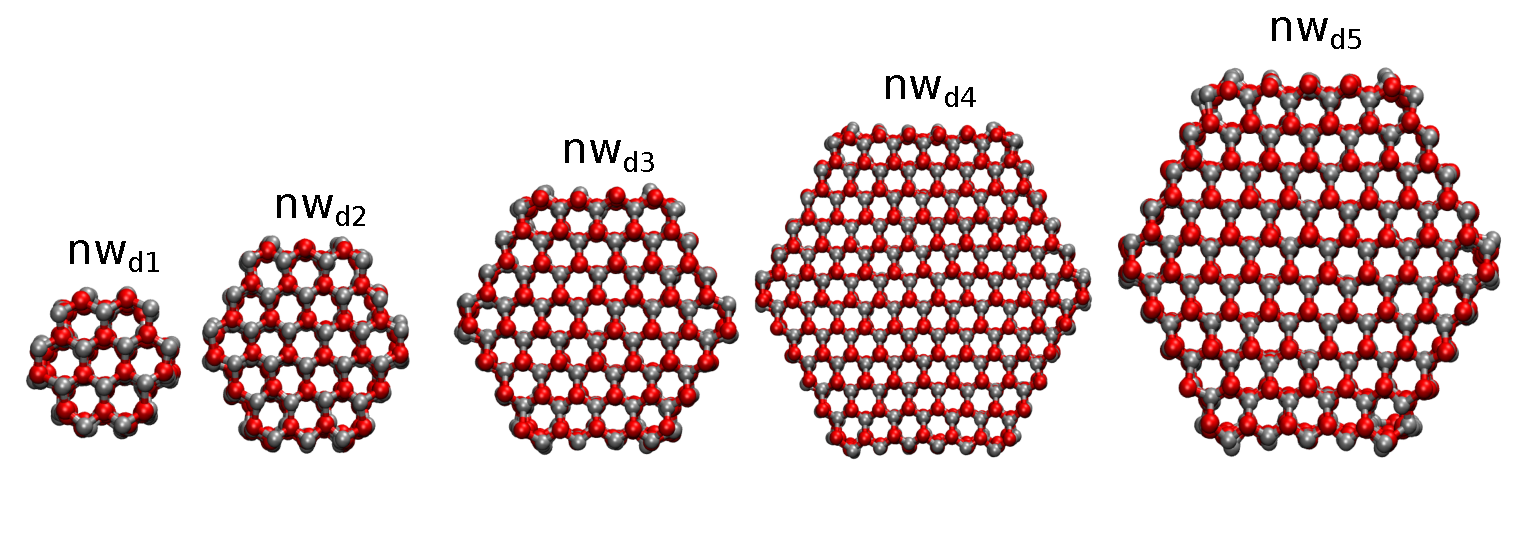
\includegraphics[height=5cm]{cap6/figs/anchos.eps}
\caption{Nw luego de realizar simulaciones de sistemas 1slv agua-nw con LAMMPS a 300 K. Los diámetros para cada nw son: $10.48$ {\AA} (nw$_{d1}$), $16.99$ (nw$_{d2}$), $23.36$ {\AA} (nw$_{d3}$), $30.33$ {\AA} (nw$_{d4}$) y $36.79$ {\AA} nw$_{d5}$.} 
\label{anchos}
\end{figure}



\begin{figure}[h!]
\centering
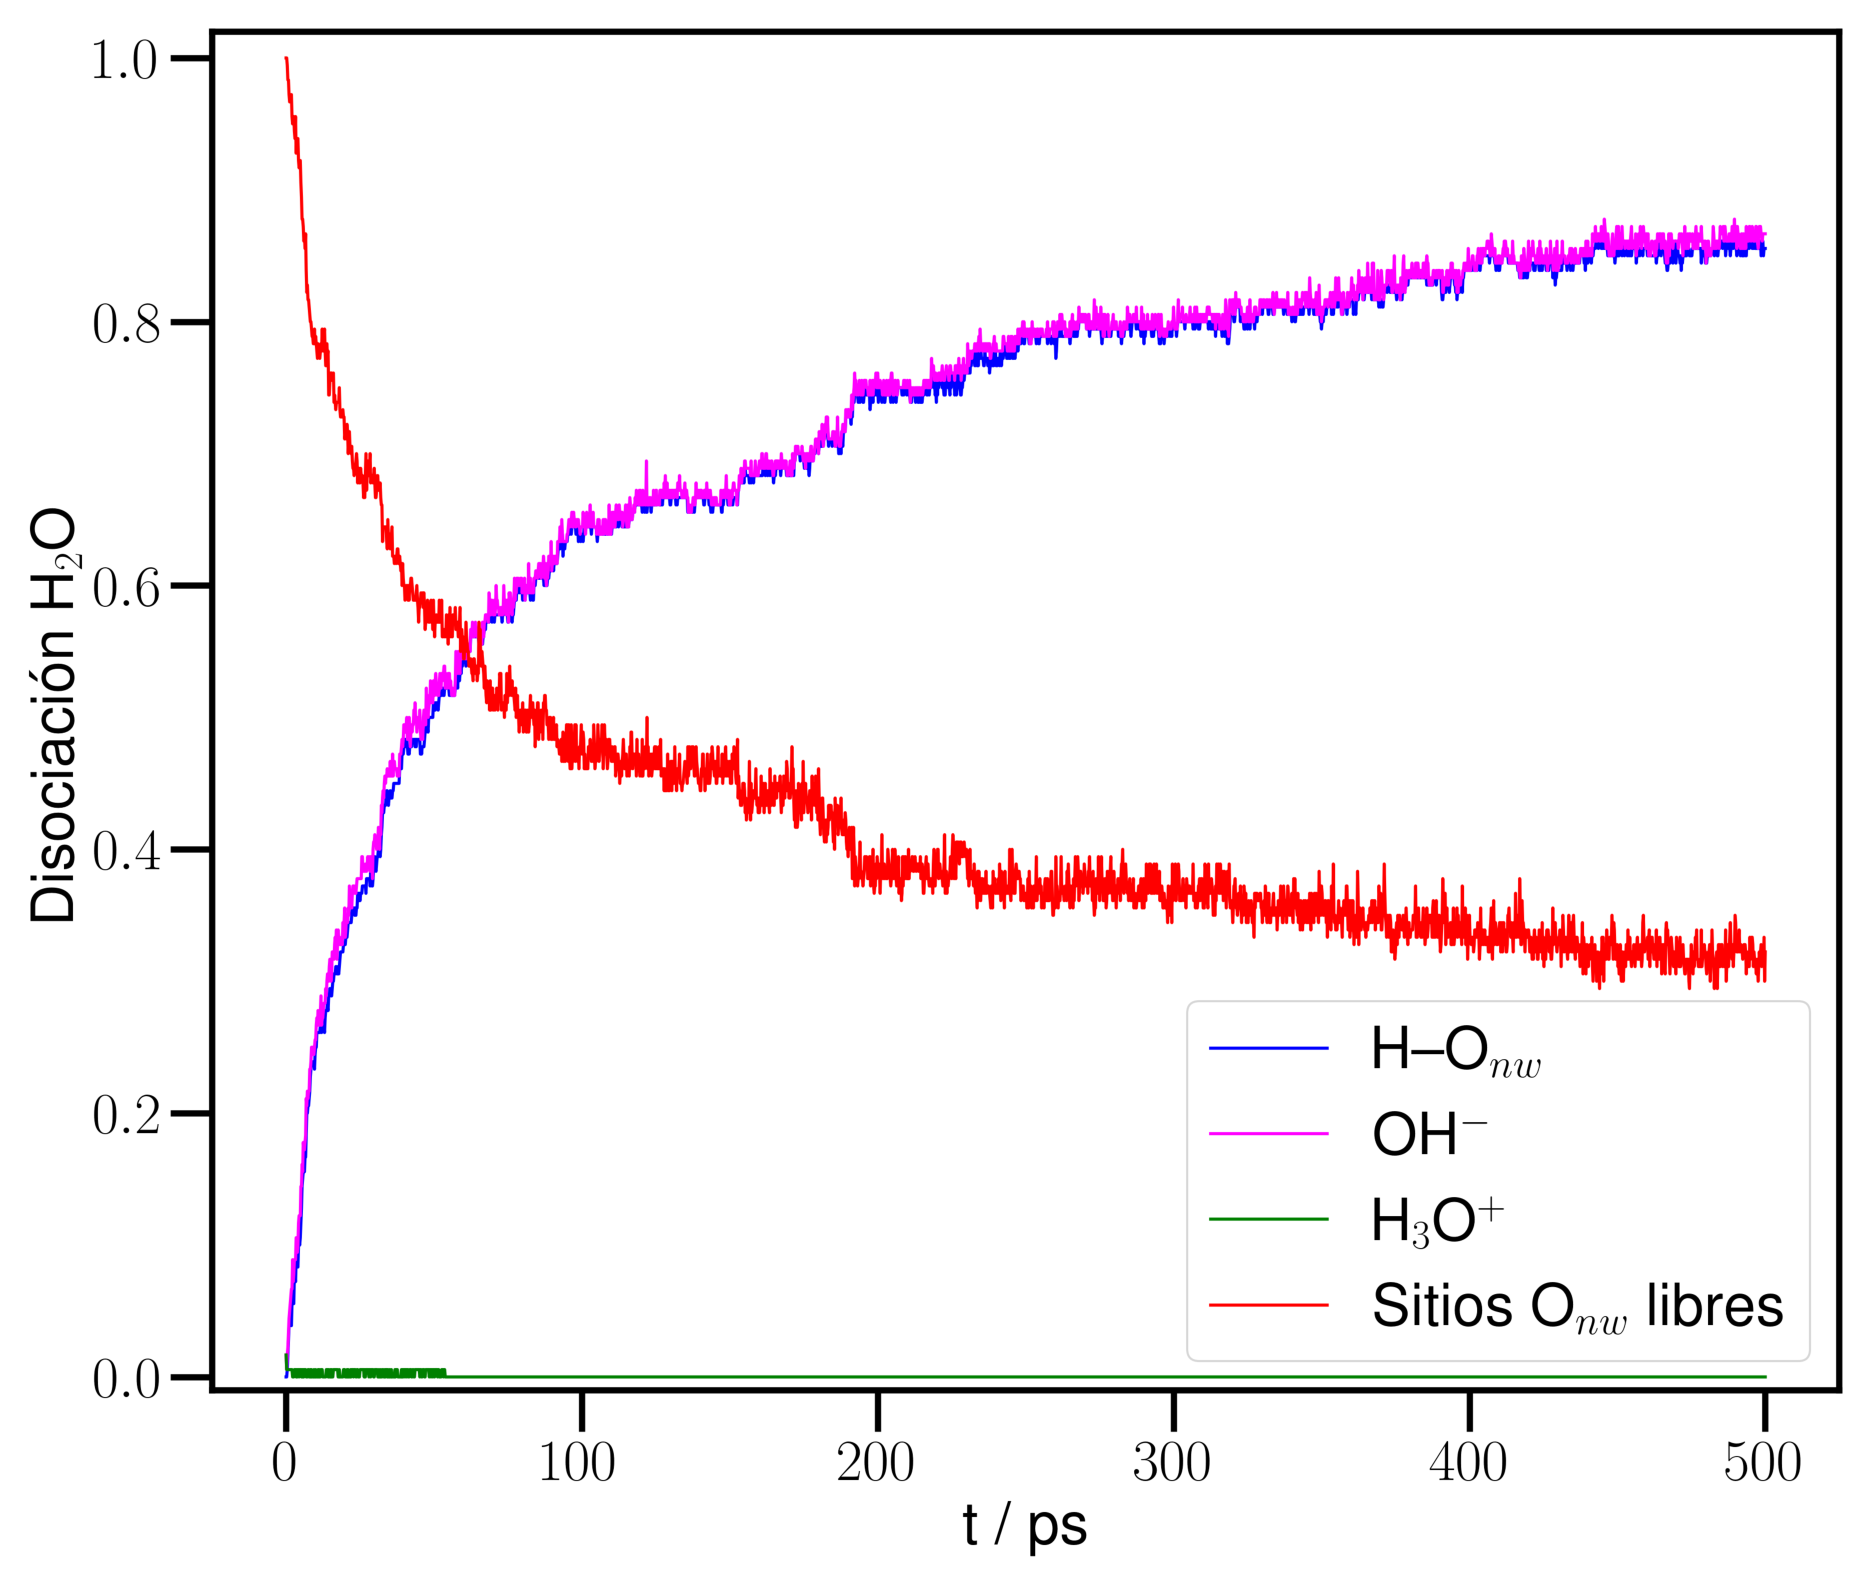
\includegraphics[height=6cm]{cap6/figs/prom_1.eps}
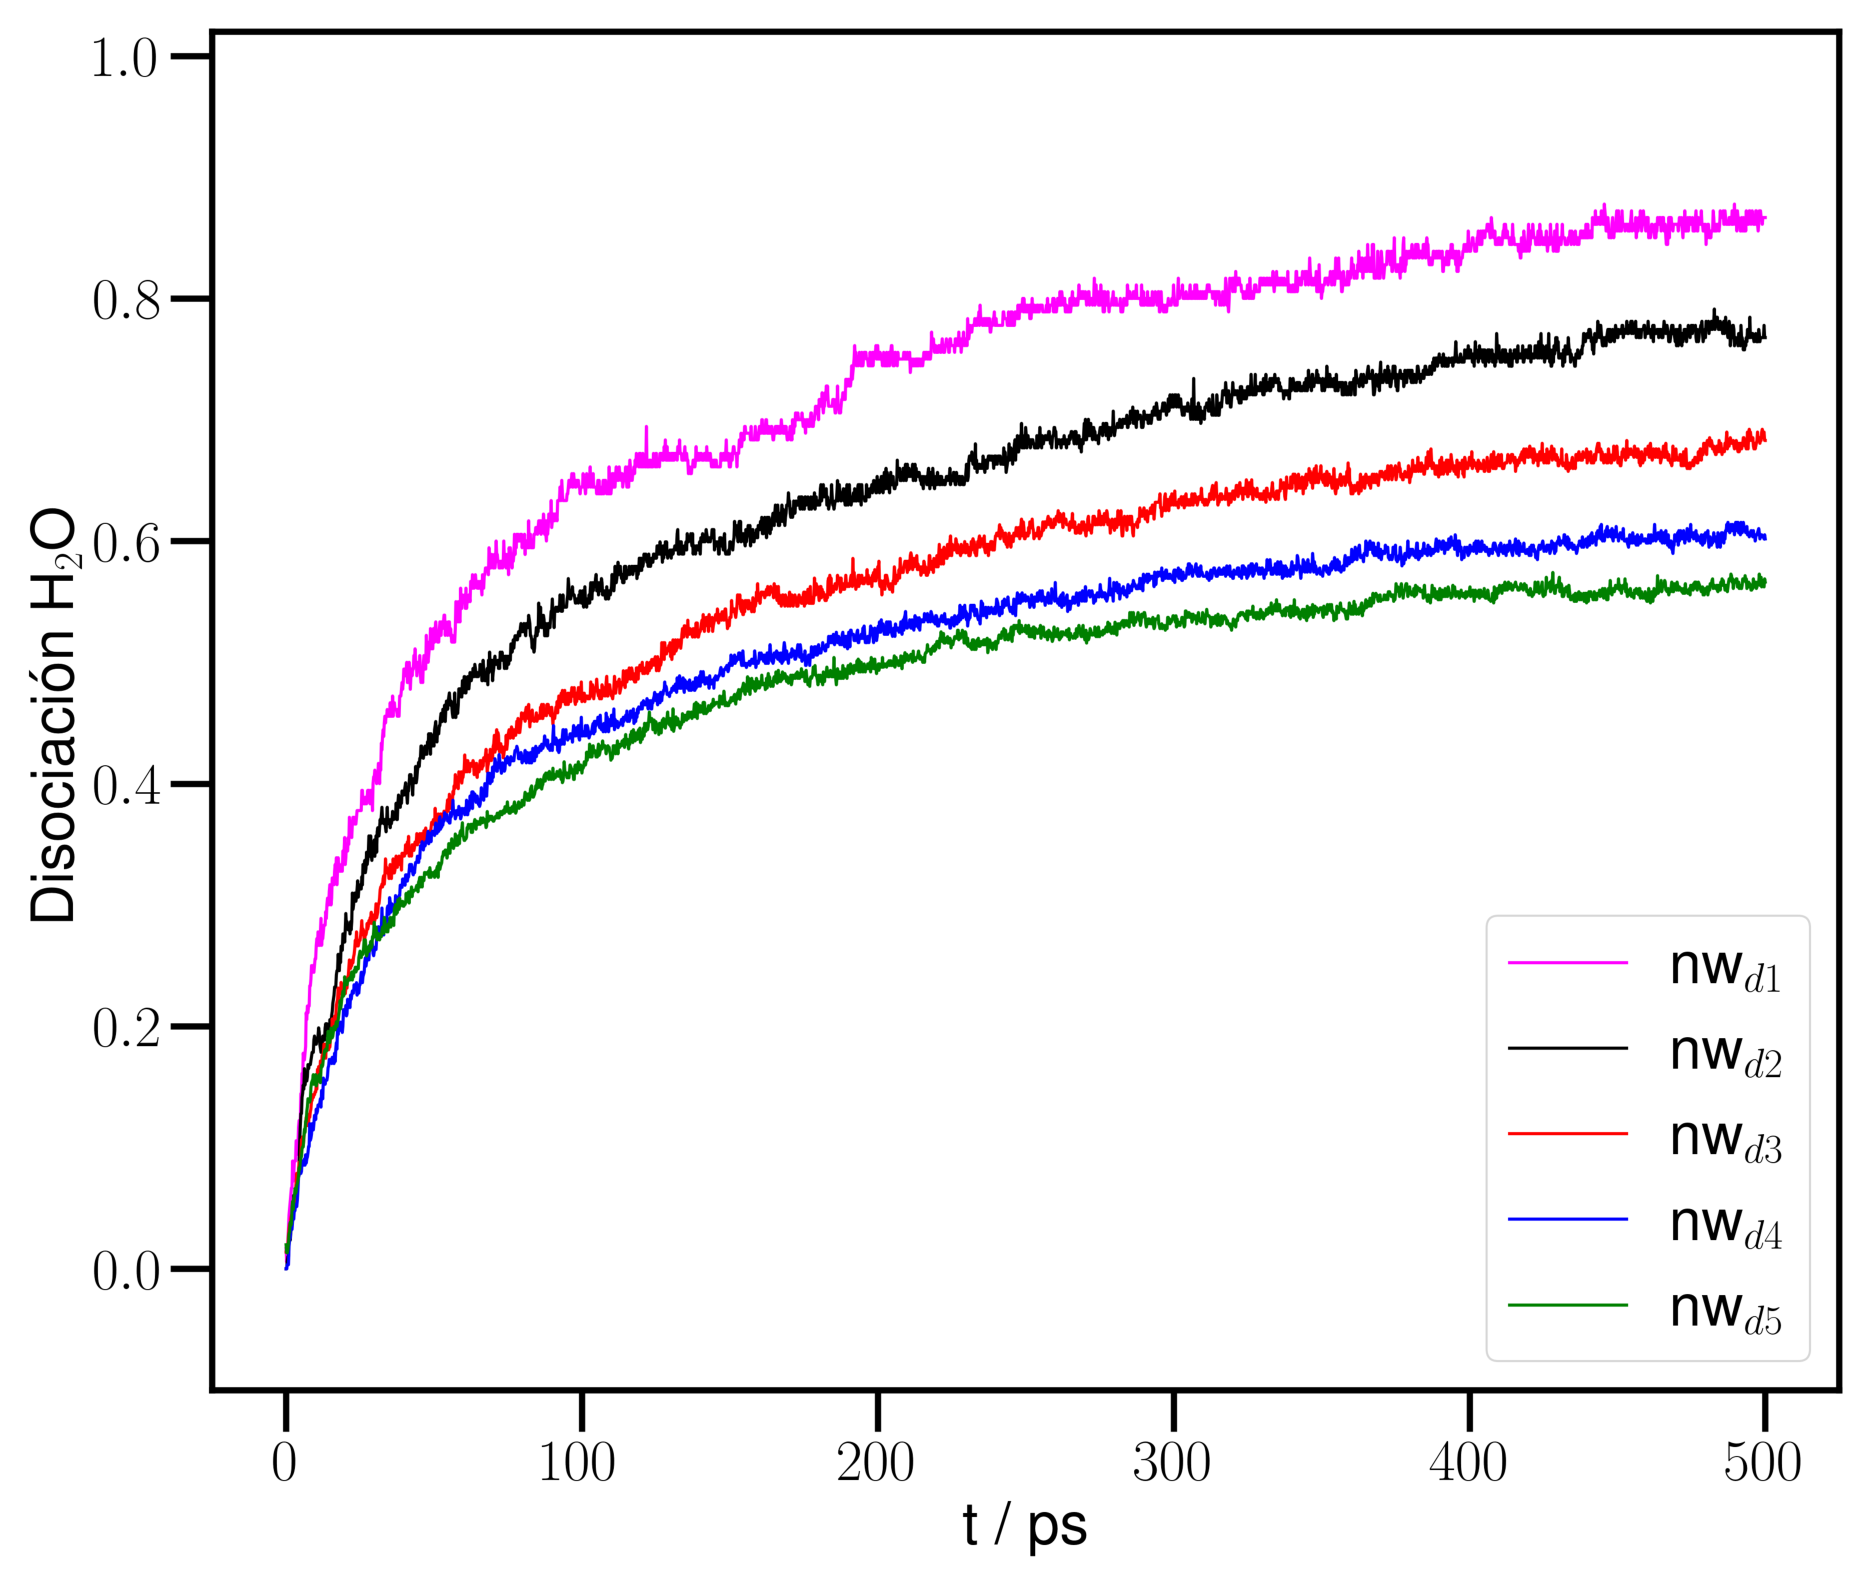
\includegraphics[height=6cm]{cap6/figs/comparacion_anchos.eps}
\caption{(\textbf {Izquierda}) Disociación de agua para el sistema 1slv agua-nw$_{d1}$ y (\textbf {derecha}) disociación de agua por unidad de superficie (1 = toda la superficie del nw) para nw con distintos diámetros} 
\label{anchos_dis}
\end{figure}

En el gráfico de la izquierda se observa la proporción de disociación para el menor diámetro (nw$_{d1}$) entre los 5 analizados. Se realizó el mismo gráfico para todos los nw obteniendo resultados muy similares cualitativamente. A medida que avanza la dinámica comienzan a disociarse las moléculas de agua generando enlaces H$_w$-O$_{nw}$ y iones OH$^-$ tal como muestran las curvas azul y rosa, respectivamente. La relación entre los productos de la disociación es 1:1 por lo que ambas curvan se muestran idénticas. A tiempos cortos las moléculas se disocian con mayor rapidez debido a que la superficie del nw cuenta con todos los sitios de O disponibles para que ocurra la reacción mientras que a tiempos largos los sitios libres comienzan a ocuparse y por ende las disociaciones son menos frecuentes. La evolución temporal de los sitios de O superficiales libres del nw (O$_{nw}$) se muestra en la curva roja, de la cual observamos que a 100 ps, la mitad de los sitios disponibles ya han sido ocupados. Por último con la curva verde nos aseguramos de que no se forman iones H$_3$O$^+$

En el gráfico de la derecha se representa la proporción de disociación de agua por unidad de superficie para los 5 diámetros elegidos. El hecho de que el cálculo sea por unidad de superficie nos permite comparar las curvas unas con otras. Cuando el nw tiene menor diámetro hay una mayor proporción de disociación de agua, es decir que ocurren más disociaciones con respecto al total posible en comparación a otros de mayor diámetro. En este caso nw$_{d1}$ es el que presenta menor diámetro y en consecuencia una mayor proporción de disociación. Se debe destacar que nw$_{d1}$ también muestra una mayor velocidad de proporción de disociación en relación a los otros nw más anchos (ver curva rosa).


\section{Conclusiones}

Validamos dftb+ configuracionalmente?

Validamos el potencial ReaxFF termodinámicamente y cinéticamente a través del cálculo de Ead y Ea

El nw cataliza la disociación del agua Ea = 0.073 eV

Cuanto mas pequeño es el alambre mayor es la proporción de disociación


